\section*{Proposal overview}

The goal of  \projacro\ is to investigate the accelerated nature of 
the expansion of our Universe 
with observations of galaxy density and peculiar velocity fields. 
We aim at measuring the growth rate of structures, quantity that 
can probe dark energy 
models and deviations from general relativity on cosmic scales. 

Our team will use state-of-the-art galaxy and supernova datasets from 
the Dark Energy Spectroscopic Instrument (DESI) and 
the Zwicky Transient Facility (ZTF), producing the best density and 
peculiar velocity fields in the Northern sky. 

\projacro\ is divided in three major components:
\begin{enumerate}
  \item \textbf{Simulations:} producing large samples of synthetic versions of DESI and ZTF surveys; 
  \item \textbf{Systematics:} quantifying the impact of observational systematics in real 
  and synthetic datasets;
  \item \textbf{Cosmology:} obtaining cosmological constraints on dark energy and 
  modified gravity theories. 
\end{enumerate} 

The optimal and unique combination of DESI densities and DESI+ZTF velocities 
is expected to yield 8.3\% precision on the growth rate at late cosmic times. 
Combined with other growth rate measurements, \projacro's results have the potential 
to reduce uncertainties on the gravitional index $\gamma$ by a factor of two. 

Our local team has the required expertise and has acquired international recognition 
in this field over recent years, and will work hand-in-hand with experts from DESI and ZTF collaborations.

The success of \projacro\ will critically depend on the workforce in our team
required to merge efforts across datasets and collaborations. 
Therefore we request funds to hire one PhD student and one 
experienced postdoctoral researcher to achieve the objectives of \projacro.

\small
\begin{center}
  \textbf{\projacro's team members \\ \ \\}

\begin{tblr}{
    width=\linewidth,
    colspec={%X[l,valign=m,wd=1.cm]
             X[l,valign=m,wd=2cm]
             X[l,valign=m,wd=2cm]
             X[l,valign=m,wd=2.cm]
             X[l,valign=m]
             X[r,valign=m,wd=3cm]},
    row{1}={font=\bfseries},
     hline{3,4,5,6,7,8,9,10, 11} = {solid,gray}
}
\hline
\hline 

Last Name &
First name &
Current position &
Role and responsibilities in the project &
{Involvement\\(person.month)} \\

\hline
\hline

Bautista &
Julian &
Professor &
Scientific coordinator &
43.2 \\

Fouchez &
Dominique &
Researcher &
Expert in supernova cosmology. All WPs &
4.8 \\


Racine &
Benjamin &
Researcher &
Expert in supernova cosmology. All WPs &
4.8 \\


Feinstein &
Fabrice &
Professor &
Expert in supernova cosmology. WP2 &
19.2 \\


Mena-Fernandez &
Juan &
Postdoc &
Expert in clustering, simulations and lensing. WP1, WP3 &
14.4 \\

Hanser &
Corentin &
Postdoc &
Expert in CMB and peculiar velocities. WP1, WP2 &
14.4 \\

Kebadian &
Rafael &
PhD student &
Expert in peculiar velocities with SNIa. WP1 and WP2.&
14.4 \\

\SetCell [c=2]{l} \textbf{To be recruited} &
 &
\textbf{PhD student} &
WP1 and WP2 &
36 \\

\SetCell [c=2]{l} \textbf{To be recruited} &
 &
\textbf{Postdoc} &
All WPs &
36 \\

\end{tblr}
\end{center}
\normalsize

\newpage

\section{Proposal's context, positioning and objective(s)}

%\emph{This paragraph refers to the evaluation criterion ``Quality and scientific aim''. }

%\emph{The criterion « Quality and scientific ambition» will be the determining one: only the 
%projects having received an « A » will proceed to the second step of the evaluation process}

%blabla with\supercite{Dumur2015} and also Ref.~\cite{Dumur2021}



\subsection{Objectives and research hypotheses}
 
The accelerated nature of the expansion of our Universe remains one of the most 
mysterious puzzles in Physics, %\cite{riessObservationalEvidenceSupernovae1998,perlmutterMeasurementsOmegaLambda1999}, 
well consolidated by several recent and 
independent cosmological observations 
\cite{planckcollaborationPlanck2018Results2020,
broutPantheonAnalysisCosmological2022,
rubinUnionUNITYCosmology2025,
descollaborationDarkEnergySurvey2024,
desicollaborationDESIDR2Results2025}.
Explanations for such an acceleration require Physics beyond our standard model 
and/or ambitious modifications of our current theory of gravity: 
general relativity.

\subsubsection*{Dark energy} 

One of the potential solutions is to introduce a new exotic component of our Universe:
 \textbf{dark energy}. 
Dark energy has negative relativistic pressure, therefore acting as 
a source of anti-gravity, repelling galaxies on large cosmic scales. 
The simplest form of dark energy is equivalent to Einstein's cosmological constant $\Lambda$. 
The cosmological constant corresponds to a fluid with an equation of state  $w = -1$ 
(relation between relativistic pressure and energy density), constant with time.  
Current observations require that at least 68\% of our Universe's energy budget is 
in form of dark energy. Such a model is dubbed $\Lambda$CDM, where CDM stands 
for cold dark matter.
More exotic dark energy models predict different values for $w$, with the only constrain 
that $w < -1/3$ to produce an accelerated expansion.  
A generalised model considers the equation of state of dark energy to be 
an time-evolving quantity
\cite{chevallierAcceleratingUniversesScaling2001,linderExploringExpansionHistory2003}, 
which can be written as $w(a) = w_0 + w_a(1-a)$, where $a$ is the scale factor 
of the Universe 
($a=1$ today and $a=0$ at the Big Bang) and $w_0, w_a$ two fixed parameters.
Such a model is referred to as $w_0w_a$CDM.  
In 2024, a combination of several cosmological measurements (see below) 
showed strong preference for an $w_0w_a$CDM Universe over a $\Lambda$CDM one by  
more than 3$\sigma$  
\cite{desicollaborationDESIDR2Results2025}, showing hints of new Physics 
for the first time since the discovery of the acceleration in the 2000's. 

\subsubsection*{Modified gravity}

An alternative solution to explain the accelerated expansion of the Universe 
is to propose alternatives to general relativity (GR) to describe gravity on large cosmic 
scales. Those are referred to as \textbf{modified gravity theories}. 
Modified gravity effects have to manifest only on cosmic scales where 
the expansion is observed, 
since GR is compatible with extremely high-precision measurements made on Earth 
\cite{poundEffectGravityNuclear1964,
hafeleAroundtheWorldAtomicClocks1972,
hafeleAroundtheWorldAtomicClocks1972a,
vessotTestRelativisticGravitation1980,
kapnerTestsGravitationalInverseSquare2007}
in the Solar System 
\cite{shapiroFourthTestGeneral1971,
titovDeflectionLightInduced2015}, 
on stars 
\cite{joyceGravitationalRedshiftSirius2018,
gravitycollaborationDetectionGravitationalRedshift2018}, 
on binary and triple systems of pulsars
\cite{taylorNewTestGeneral1982,
stairsTestingGeneralRelativity2003,
kramerTestsGeneralRelativity2006,
voisinImprovedTestStrong2020}, 
as well as 
in mergers of black holes and neutron stars 
\cite{theligoscientificcollaborationObservationGravitationalWaves2016,
theligoscientificcollaborationGW170817ObservationGravitational2017}. 
Direct imaging of black holes also are consistent
with GR, in a very strong field regime 
\cite{eventhorizontelescopecollaborationFirstM87Event2019}.
There are several families of models trying to extend or modify GR 
to account for 
the observed acceleration of the Universe 
\cite{cliftonModifiedGravityCosmology2012,
zhaiClusteringLuminousRed2017,
ezquiagaDarkEnergyLight2018,
ferreiraCosmologicalTestsGravity2019,
houCosmologicalProbesStructure2023}.
However, such models predict the same \textit{expansion history} as dark energy, 
so we need an alternative observable to discriminate between dark energy and 
modified gravity models. One of the best observables is 
the \textit{growth history} of 
the cosmic density field of the Universe
and its impact on its velocity field. 

\subsubsection*{Expansion rate and distance indicators}

The expansion rate of the Universe, $H(z)$, as a function of time or redshift $z$, 
has been historically been measured via the average distance-redshift relationship 
of extragalactic objects. 
Redshifts are precisely measured with spectroscopy, but distances are  
a more challenging endeavour. 
Several distance indicators have been used
in recent years: 
the Tully-Fisher (TF, \cite{tullyNewMethodDetermining1977}) 
and Fundamental Plane (FP, \cite{djorgovskiFundamentalPropertiesElliptical1987}) 
relations, as well as 
type-Ia supernovae (SNIa, \cite{kowalAbsoluteMagnitudesSupernovae1968}). 
The first two indicators (TF and FP) rely on empirical relations between galaxy properties 
and their luminosity or size, so in principle they can be applied large samples of galaxies. 
However those relations have a large intrinsic scatter of about 20-30\% in distances 
compared to SNIa (5-10\%). SNIa are more precise distance indicators but are less numerous than TF and FP galaxies
The discovery of the accelerated expansion in the 2000's used samples of tens of SNIa
\cite{riessObservationalEvidenceSupernovae1998,perlmutterMeasurementsOmegaLambda1999}
while today's samples reach several thousands (see below).
%Measurements of today's expansion rate, $H_0$, from late time probes are currently 
%in strong tension ($> 5\sigma$) with early time probes. 
\textbf{\projacro\ will employ state-of-the-art samples of 
distance indicators to constrain models of dark energy and modified gravity.}

%\textbf{The main goal of \projacro\ is to produce robust measurements of the growth rate of structures
%at late cosmic times (when acceleration is taking place) by using state-of-the-art 
%observations of our Universe.}
%While modified gravity theories predict the same expansion rate as dark energy, 
%its signature consists in predicting a different growth rate than dark energy. 
%The growth rate can be expressed 
%as $f(z) = [\Omega_m(z)]^\gamma$, where $\Omega_m(z)$ 
%is the fraction of matter in the Universe and $\gamma$ is the growth index.%\cite{linderParameterizedBeyondEinsteinGrowth2007}. 
%In GR, the growth index $\gamma=0.55$, while in modified gravity theories it takes 
%different values. 
%\textbf{\projacro\ will constrain the dark energy equation of state as well as potential deviations 
%from general relativity by measuring the growth rate of structures.}

\begin{figure}[t]
  \centering
  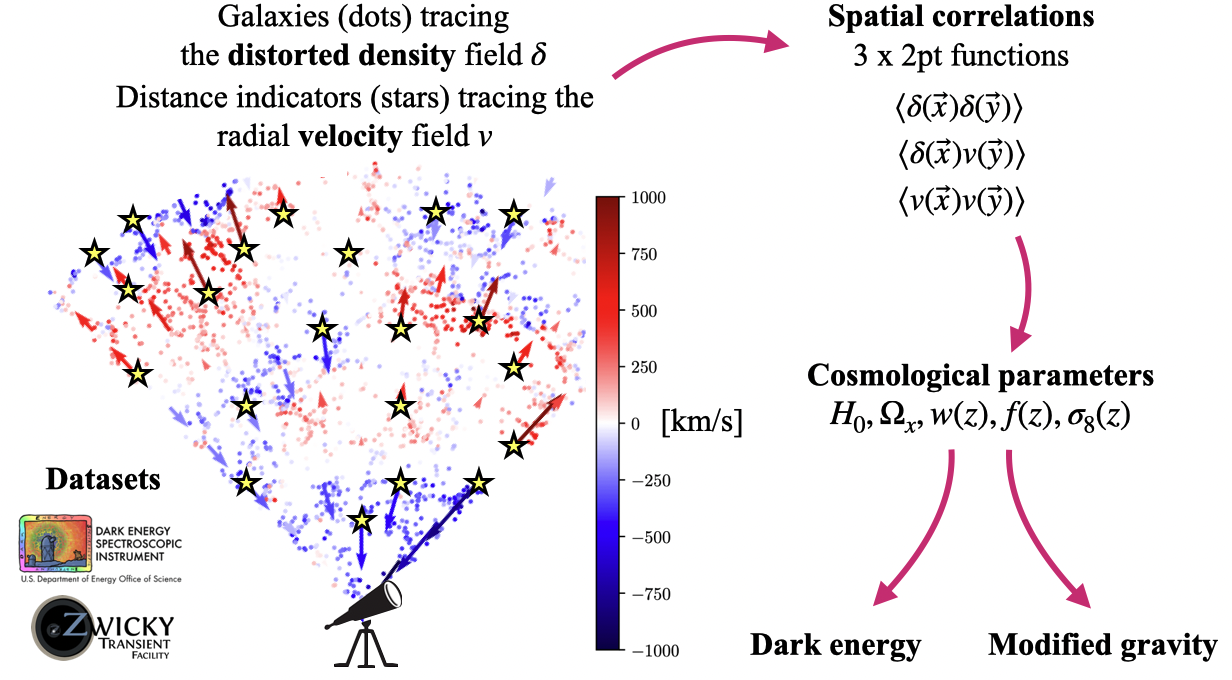
\includegraphics[width=0.8\textwidth]{figures/cosmopv.png}
  \caption{Schematic view of the \projacro. 
  We will use state-of-the-art samples of galaxy redshifts and 
  distance indicators to measure both the distorted density field 
  and the radial peculiar velocity field to derive better constraints on 
  the growth rate of structures, dark energy and modified gravity theories.}
  \label{fig:cosmopv}
\end{figure}

\subsubsection*{Growth rate of structures and peculiar velocities}

The growth rate of structures $f(z)$ quantifies how fast initial perturbations of the 
cosmic density field, $\delta(\vec{x})$, grow with time or decreasing redshift $z$. 
The r.m.s. of the cosmic density field smoothed on scales of 8\hmpc\ noted 
$\sigma_8(z)$ also 
quantifies structure growth versus time. 
The product $f(z) \sigma_8(z)$ can be measured via the impact of 
\emph{peculiar velocities} of galaxies on the observed structures. 
Peculiar velocities (PV) are simply the motions of galaxies 
due to gravitational attraction from dense structures, therefore 
they are important to test gravity on cosmic scales. 
PVs modify redshifts due to the cosmic expansion. 
Both are generally undistiguishable, creating distortions in the 
observed galaxy density field, known as \emph{redshift-space distortions} (RSD). 
The two-point statistics of the galaxy density field, $\langle \delta(\vec{x}) \delta(\vec{y})\rangle$, 
becomes anisotropic w.r.t. the line of sight, allowing measurements of the growth rate $f(z)$ 
with spectroscopic galaxy surveys 
\cite{alamClusteringGalaxiesCompleted2017,
alamCompletedSDSSIVExtended2021,
desicollaborationDESI2024FullShape2025}.
Moreover, if distance indicators are available for a large sample of galaxies,
it is possible to break the degeneracy between velocity due to cosmic expansion and  
velocity due to proper motion. 
Measuring the velocity field $v(\vec{x})$ brings extra information 
than just measuring the distorted galaxy density field $\delta(\vec{x})$. 
The two-point statistics of the velocity field, 
$\langle v(\vec{x}) v(\vec{y})\rangle$, also depends on $f(z)\sigma_8(z)$.
Measuring three combinations of two-point functions, i.e., 
density-density, velocity-velocity and their cross correlation
 $\langle \delta(\vec{x}) v(\vec{y})\rangle$,
yield tighter constraints than just one of such statistics 
\cite{qinRedshiftspaceMomentumPower2019,
%adamsJointGrowthrateMeasurements2020,
%saidJointAnalysis6dFGS2020,
turnerLocalMeasurementGrowth2023,
boubelLargescaleMotionsGrowth2024,
qinRedshiftspaceMomentumPower2025}.
Figure~\ref{fig:cosmopv} shows a schematic view of such a combination. 
\textbf{\projacro\ will employ state-of-the-art samples of distance indicators (FP, TF, and SNIa)
to measure peculiar velocities and obtain the 
tightest constraints on the growth rate in the nearby Universe.} 

\newpage 

\subsection{Position of the project in relation to the state of the art}
\label{sec:state-of-the-art}

  \projacro\ is timely because it will profit from state-of-the-art datasets to 
produce robust measurements of the growth rate of structures. Our team members
are active members of the Dark Energy Spectroscopic Instrument (DESI) and 
the Zwicky Transient Facility (ZTF), and have the required expertise to achieve
\projacro's goals. 

\subsubsection*{The Dark Energy Spectroscopic Instrument (DESI)}

  Currently the best spectroscopic survey of galaxies, 
  DESI will measure 63 million galaxy redshifts after eight 
  years of observations (2021-2028) over 17,000~deg$^2$ 
  \cite{desicollaborationOverviewInstrumentationDark2022}. 
  DESI observes galaxies and quasars, which serve as excellent 
  tracers of the distorted matter density field. 
  By analyzing these redshift-space distortions (RSD), 
  we can infer the growth rate of cosmic structures. 
  The growth rate measurements from DESI Data Release 1 (DR1) 
  \cite{desicollaborationDataRelease12025}
  were published in 2024 
  \cite{desicollaborationDESI2024FullShape2025}
  as well as their cosmological implications 
  \cite{desicollaborationDESI2024VII2025,
  forero-sanchezCosmologicalConstraintsJoint2026}.
  Such growth rate measurements are displayed as red points in Figure~\ref{fig:fs8} at $z>0.1$.

\subsubsection*{DESI Peculiar Velocity Survey and recent results}

  The DESI Peculiar Velocity survey is a secondary program 
  that will produce, when completed, distance measurements to 
  53k spiral galaxies from the Tully-Fisher relation and 133k ellipticals 
  from the Fundamental Plane 
  \cite{saulderTargetSelectionDESI2023, 
  saidDESIPeculiarVelocity2024,
  douglassDESIEDRCalibrating2025}.
  Those distances will yield a well sampled velocity field at $z<0.1$, 
  perfectly overlapping with the DESI Bright Galaxy sample 
  \cite{hahnDESIBrightGalaxy2022}, which provides an excellent density field. 

  Since 2024, the scientific coordinator of \projacro\ was nominated 
  as co-chair of the DESI Transients and Low-z cosmology working group, 
  responsible for the Peculiar Velocity survey. Since then, we are 
  actively involved in the organisation and execution of the growth 
  rate measurement with such data. 
  In December 2025, we released a batch of seven publications 
  describing the growth rate measurements with DESI DR1. 
  We report a 12.5\% measurement of $f(z) \sigma_8(z)$ at $z=0.07$ 
  \cite{bautistaDESIDR1Peculiar2025,
  douglassDESIDR1Peculiar2025,
  carrDESIDR1Peculiar2025,
  qinDESIDR1Peculiar2025,
  rossDESIDR1Peculiar2025,
  turnerDESIDR1Peculiar2025}. 
  
  The scientific coordinator was first author of the publication 
  describing the simulated datasets \cite{bautistaDESIDR1Peculiar2025}. 
  Those simulations represent the largest and most accurate set  
  for peculiar velocity studies so far, including 675 realisations 
  of DESI DR1 galaxy and peculiar velocity samples. It was based 
  on the AbacusSummit suite of n-body simulations 
  \cite{maksimovaABACUSSUMMITMassiveSet2021} and 
  an evolving halo occupation distribution model
  \cite{smithGeneratingMockGalaxy2024}.
  \textbf{In \projacro, we will build upon this expertise to produce larger and 
  better samples of simulated data (Work Package \ref{sims}).}

  We were also lead authors of the growth rate measurement with 
  the momentum power spectrum method 
  \cite{qinDESIDR1Peculiar2025}.
  This method is one of the three used with the same data, besides 
  the maximum likelihood estimator \cite{laiDESIDR1Peculiar2025}
  and correlation functions \cite{turnerDESIDR1Peculiar2025}. 
  In those analyses, some unexplained systematic effects were found.
  First, the Tully-Fisher data 
  at $0.05< z <0.10$ shows spurious correlations, so they were 
  excluded from our baseline analysis. 
  Second, residual spurious correlations persist in the final catalog, 
  primarily affecting small scales, which motivated the application 
  of a scale cut to the momentum auto-power spectrum.
  \textbf{Within \projacro, we will address these systematic effects 
  by investigating their origin, correcting them when possible, 
  and quantifying their impact on the growth rate of structures 
  (Work Package \ref{systematics}).}

  
\subsubsection*{The Zwicky Transient Facility (ZTF)}

  ZTF is a photometric survey with large field of view and high cadence, ideal for the 
  discovery of transient events, including SNIa 
  \cite{bellmZwickyTransientFacility2019}.
  Covering the whole sky down to declination of -30$^\circ$ 
  and perfectly overlapping with DESI observations, 
  ZTF discovered more than 30k SNIa over redshifts $0 < z < 0.2$, 
  which will be used for cosmological studies. 
  More than 5k SNIa were spectroscopically
  classified by ZTF or other telescopes. 
  ZTF observations ran from 2017 to 2023, 
  and now the ZTF collaboration, including members of \projacro, are working on 
  an improved pipeline optimized for precision cosmology and dark energy studies, 
  including the measurement of the growth rate from SNIa peculiar velocities.  
  The ZTF Data Release 2 \cite{rigaultZTFSNIa2025} contains half of the observations
  and is the last public release of ZTF data.

\subsubsection*{ZTF peculiar velocities and recent results}

  Preliminary work on simulations started at CPPM to quantify the potential 
  for cosmological measurements with ZTF SNIa sample. 
  We developed an analysis
  pipeline for 1) simulating realistic observations of ZTF SNIa, a package 
  called \textsc{SNSIM}\footnote{\url{https://snsim.readthedocs.io}} and 2) 
  measuring the growth rate of structures with ZTF SNIa peculiar velocities 
  using the maximum likelihood estimator
  \cite{carreresGrowthrateMeasurementTypeIa2023}. This pioneering work 
  in ZTF predicts an uncertainty of 17\% on the growth rate 
  from SNIa peculiar velocities only, without a galaxy density field 
  (Figure~\ref{fig:fs8}). 

  We generalized this pipeline to include cross correlations 
  with a distorted galaxy density field, correctly accounting for non-linear clustering 
  and wide angle effects. This new framework is called Field Level Inference Package 
  (\textsc{FLIP}, \cite{ravouxGeneralizedFrameworkLikelihoodbased2025}) and is publicly 
  available\footnote{\url{https://flip.readthedocs.io}}.
  Thanks to several numerical optimizations as well as the implementation of emulators, 
  FLIP was used to quantify the potential for growth rate measurements 
  with the Vera Rubin Observatory \cite{rosselliForecastGrowthrateMeasurement2025},
  which contains one order of magnitude more SNIa. 

  \textbf{\projacro\ will build upon this expertise with SNIa peculiar velocities 
  and apply it to the cosmology sample of ZTF SNIa.} We will produce simulations
  of ZTF with improved realism (Work Package \ref{sims}) and use them to quantify biases and 
  systematic errors in real data (Work Package \ref{systematics}). 
  
  While ZTF DR2 concerns the spectroscopically confirmed sample of SNIa, 
  there is also a huge potential to increase numbers and redshift range 
  by employing a photometrically-classified sample of SNIa. This sample is
  4 to 5 times larger than the spectroscopically-classified sample, 
  and reaches redshifts up to $z < 0.2$. WP2 of \projacro\ also will 
  explore this opportunity to improve growth rate measurements.


\begin{figure}[t]%{r}{0.6\textwidth}  
 \centering
  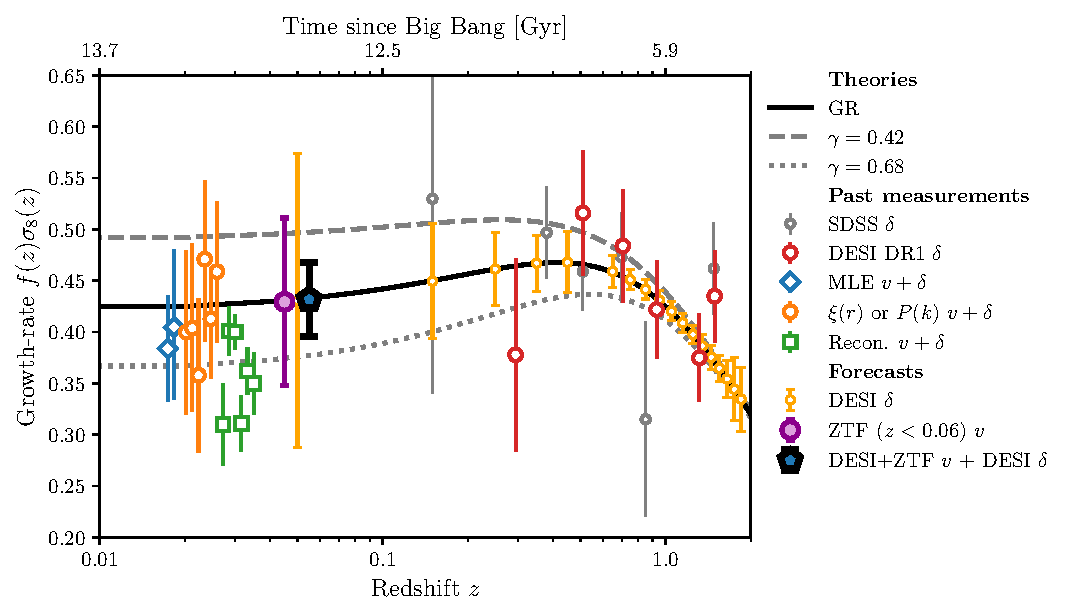
\includegraphics[width=0.9\textwidth]{figures/fs8_theory_sdss_desiy1_desi_pv_ztf_ztfdesi_english.pdf}
  \caption{Growth rate of structures versus redshift from past measurements compared to expected results from  \projacro, which will 
  employ low-redshift galaxies and peculiar velocities from the Dark Energy Spectroscopic Instrument (DESI) and the Zwicky Transient Facility (ZTF).}
  \label{fig:fs8}
\end{figure}


\subsubsection*{Combining DESI and ZTF peculiar velocities}

  \projacro\ will focus in the DESI and ZTF overlap, a perfect opportunity 
  for cross-correlations and systematic cross-checks, and produce a joint 
  measurement of the growth rate of structures. 
  Based on our own Fisher forecasts and analysis of simulations using FLIP
  \cite{carreresGrowthrateMeasurementTypeIa2023,
  ravouxGeneralizedFrameworkLikelihoodbased2025}, 
  \textbf{\projacro\ has the potential of producing a 
  8.3\% precision growth rate 
  measurement when combining DESI galaxies and DESI+ZTF velocities 
  (Figure~\ref{fig:fs8}), representing the most precise and robust 
  estimate at late cosmic times.} This number is to be compared to the current 
  12.5\% measurement of DESI DR1 PV only
  \cite{qinDESIDR1Peculiar2025,laiDESIDR1Peculiar2025,turnerDESIDR1Peculiar2025}. 

  Cosmological implications of such a measurement will be explored in Work Package~\ref{cosmo},
  including the standard $\Lambda$CDM model as well as extensions 
  parametrizing modified gravity theories (or departures from GR).





%Producing large samples of synthetic datasets reproducing real 
%data at high fidelity is an essential ingredient.
%Those sets have multiple uses: testing our methodologies for biases,
%understand our uncertainties, compute covariance matrices of observables, 
%and study the impact of systematic effects on cosmological results. 
%Building up on current experience in our team 
%\cite{bautistaMockQuasarLymanalphaForest2015,
%zhaoCompletedSDSSIVExtended2021,
%qinCosmicFlowMeasurement2021,
%carreresGrowthrateMeasurementTypeIa2023,
%rosselliForecastGrowthrateMeasurement2025,  
%bautistaDESIDR1Peculiar2025},
%\textbf{\projacro\ will lead the production of the most realistic 
%synthetic datasets for both DESI and ZTF (Work Package~\ref{sims})} 

%Properly combining two samples of peculiar velocities from DESI and ZTF 
%is an interesting problem. Distance indicators such as Tully-Fisher, 
%Fundamental Plane and type-Ia supernovae require a calibration from 
%lower rangs of the distance ladder such as cepheids, or distances 
%from the tip of the red 
%giant branch. 
%To obtain consistent peculiar velocities
%between surveys, such as calibration has to be done carefully. 
%Work Package~\ref{systematics} will tackle this problem. 



\subsection{Methodology and risk management}
\label{sec:method}

%\begin{footnotesize}
%Describe precisely the methodology and its relevance to reach the objectives; 
%detail the scientific risks and fallback solutions envisaged; 
%describe the scientific program and justify the breakdown of 
%the work program into tasks in line with the objectives pursued.
%
%\begin{itemize}
%  \item For each task, describe the objectives, the work programme, deliverables, 
%  contributions of the partners, methods and technical choices, risks and fallback
%   solutions (among other examples: difficulty to access study site, lack of 
%   preliminary data, delay in obtaining approval from the ethics committee, etc.). 
%   Illustrate with a Gantt chart.
%	\item Justify the relevance of the methodology in terms of ethics, scientific 
%  integrity and social responsibility of sciences - and as such, considering or 
%  not the sex and/or gender aspect , considering the ecological sustainability in the implementation of the project -, and in terms of disciplinary coverage (mono- trans- and inter-disciplinarity). 
%	\item If applicable, indicate the conditions of access to a research 
%  infrastructure IR, IR* or OSI
%\end{itemize} 
%\end{footnotesize} 


%Methodology to reach the scientific objectives of the project, 
% detailed description of the intended method(s) including its disciplinary 
% coverage (mono-trans-inter-disciplinary)

\projacro\ is organised in three connected work packages: simulations, 
systematics, and cosmology. Figure~\ref{fig:gantt} shows the timeline 
of these three WPs, their tasks and corresponding actors. 

\wpdef{sims}{Simulations}
WP1 will focus on the production and analyses of realistic synthetic datasets 
reproducing properties of real data from DESI and ZTF. 
Simulations are a key ingredient of any robust cosmological analysis and have 
several uses: testing our methodologies for biases, 
understand our uncertainties, compute covariance matrices of observables, 
and study the impact of systematic effects on cosmological results. 
This work package will push the state of the art in the production of 
synthetic datasets for both DESI and ZTF, increasing the number of realisations, 
as well as the realism of implemented observational features. 

%\tdef{fast_sims}{Fast approximate simulations}
%    Recent mock catalogs used for peculiar velocities are based on n-body simulations 
%    such as 
%    which are high accuracy but are limited in volume or in the number of independent realisations.
%    Using well-known techniques \cite{chuangEZmocksExtendingZel2015,zhaoCompletedSDSSIVExtended2021},
%    we will  
%    produce a large number ($O(1000)$) of independent realisations of density and velocity fields at low redshift. 
  
\tdef{real_sims}{Production of synthetic samples for the DESI and ZTF PV samples} 
    Based on acquired experience with mock production for the DESI Peculiar 
    Velocity survey \cite{bautistaDESIDR1Peculiar2025}
    and the ZTF SNIa sample \cite{carreresGrowthrateMeasurementTypeIa2023}, 
    we will produce larger samples of realistic mock catalogues simultaneously 
    including both surveys and their respective observational properties. 

    We will use already available suites of n-body simulations such as AbacusSummit 
    \cite{maksimovaABACUSSUMMITMassiveSet2021,} 
    or Uchuu \cite{ishiyamaUchuuSimulationsData2021,fernandez-garciaDESIDR2Reference2025}, 
    which model precisely the density and velocity field to non-linear scales. 
    
    While precise, n-body simulations are limited in volume and the number of possible 
    realizations we can obtain from them ($\mathcal{O}(100)$). 
    To achieve larger number of realisations ($\mathcal{O}(1000)$), we plan to also 
    use fast approximate simulations such as the \textsc{EZmocks} 
    \cite{chuangEZmocksExtendingZel2015,zhaoCompletedSDSSIVExtended2021}
    or GLAM mocks \cite{klypinDarkMatterStatistics2018,erezaUCHUUGLAMBOSSEBOSS2024}. 
    Larger number of realizations are important to obtain precise covariance matrices 
    and to test biases and systematic effects to higher statitical precision. 

    We will use current methods to imprint Tully-Fisher and Fundamental plane samples in 
    DESI galaxy mocks as well as realistic ZTF light-curves, including peculiar velocities. 
    By construction, those mocks will contain the cross-correlations between surveys, 
    which will be correctly accounted for when deriving cosmological constraints from a 
    joint analysis.     
    Those new mock catalogues will reach higher redshifts than current sets, 
    and will include redshift evolution of the clustering signal and galaxy properties as well as 
    selection effects. 


\tdef{cross_cov}{Cross-covariance between methodologies and cosmological probes}
    Several methodologies are able to exploit a distorted 
    density field and a peculiar velocity field 
    (e.g.  
    \cite{ravouxGeneralizedFrameworkLikelihoodbased2025,
    qinRedshiftspaceMomentumPower2025}). 
    Those are commonly applied to the same initial dataset, 
    so results are correlated. For example, DESI DR1 PV growth rate measurements from three methodologies\
    \cite{qinDESIDR1Peculiar2025,laiDESIDR1Peculiar2025,turnerDESIDR1Peculiar2025} 
    applied to the same dataset have correlations estimated around 27 and 38\% 
    thanks to mock catalogs \cite{bautistaDESIDR1Peculiar2025}.

    Using large sets of mock catalogues, we will 
    precisely estimate the cross-correlation between methodologies applied to the same data, 
    which is key to derive robust consensus results and their uncertainties
    (e.g. \cite{sanchezClusteringGalaxiesCompleted2017,
    bautistaCompletedSDSSIVExtended2021,
    dumerchatBaryonAcousticOscillations2022}).
    Using larger datasets such as DESI DR2 and DR3 and ZTF DR3 and DR4, we will 
    investigate the cross-correlation between those methods to a higher 
    statistical precision. 

    The same mocks will be also used to evaluate the cross-covariance 
    between growth measurements from peculiar velocities and 
    weak gravitational lensing, since both probes use information from 
    the same overlapping volumes. The mocks will have to include ray-tracing 
    to include the shear of background galaxies caused by the same 
    matter density field used in peculiar velocity measurements. 

\paragraph{Deliverables}
    We will deliver large sets of precise and realistic simulations for both 
    the DESI PV survey and the ZTF SNIa sample. First, they will be released 
    internally for both collaborations so all members can use them. 
    Second, they will be made available to the community for public use, after 
    publication of the final results. 

 \paragraph{Risk management} 
    
    The production of mock catalogues is a time-consuming process and requires
    available computational resources. We expect to have access to computing 
    time as our simulations are a key ingredient for both collaborations. 
    For instance the DESI collaboration provides computing time at the 
    NERSC supercomputer while ZTF provides access to the CNRS Computing Center. 
    We also have available computing ressources at CPPM, which can also be used 
    for this WP. 
    Therefore we qualify the risk of this WP to be low. 
     


\begin{figure}[t]
  \centering
  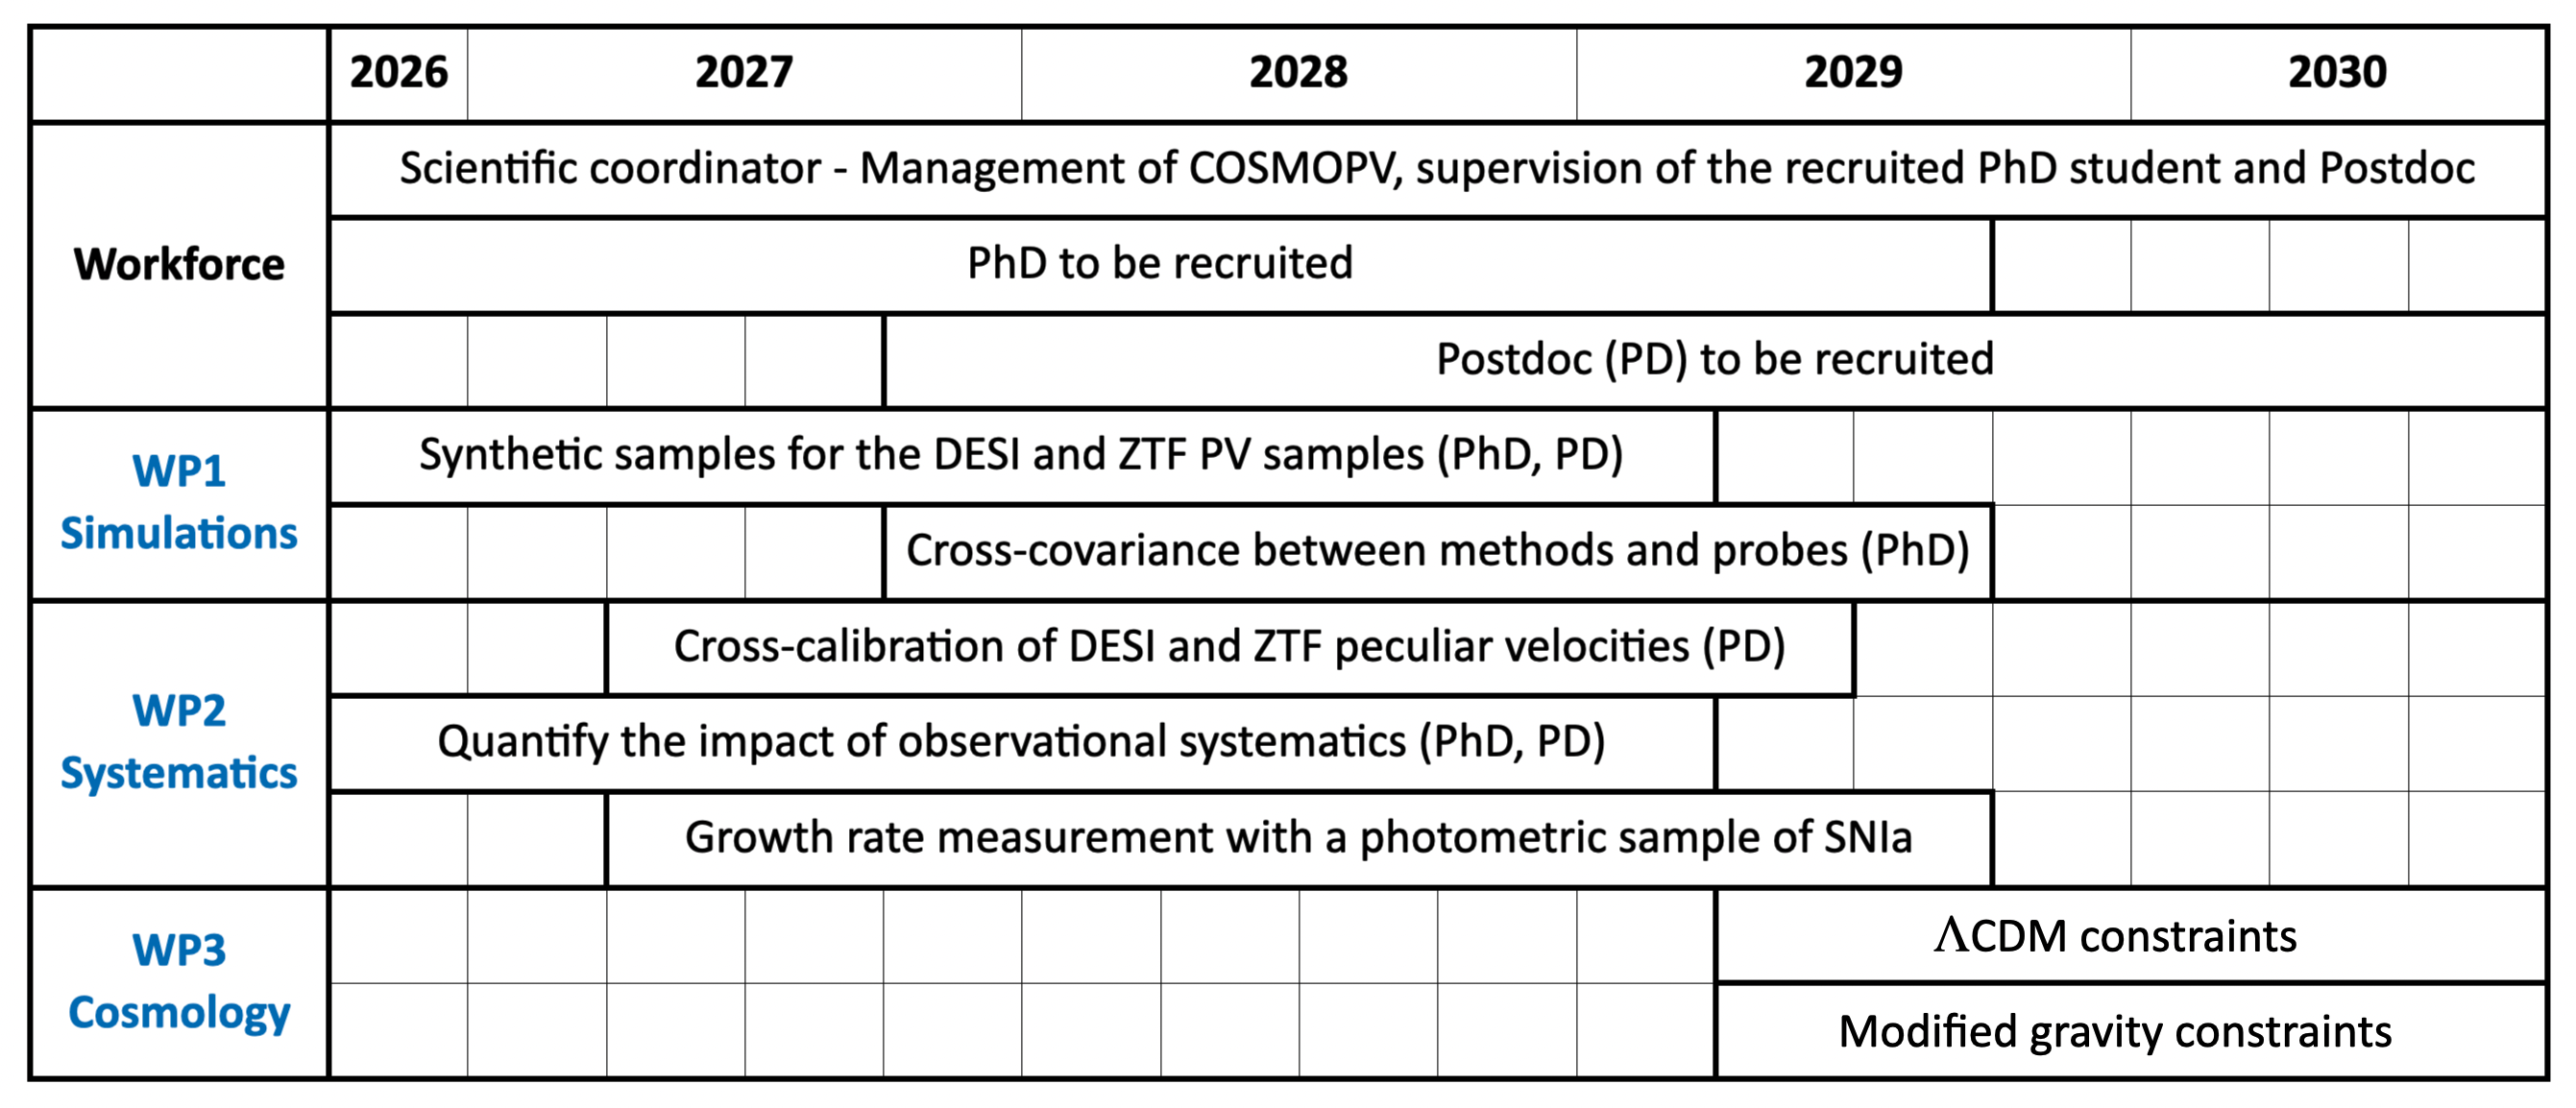
\includegraphics[width=\textwidth]{figures/gantt.png} 
  \caption{Gantt chart of the \projacro\ project.} 
  \label{fig:gantt}
\end{figure}  

\wpdef{systematics}{Systematic effects in real data}
Focusing on an interplay between real data and simulations from WP1, 
WP2 will investigate potential systematic effects 
affecting our measurents with DESI and ZTF peculiar velocities. 
We will tackle systematics both at the level of creating a joint PV catalog
after cross-calibrating both surveys, and at the level of
growth rate measurements from those PV catalogs, looking for potential 
contamination by unwanted correlations in caused by observational artifacts. 



  \tdef{cross_calib_desi_ztf}{Cross-calibration of DESI and ZTF peculiar velocities}
    DESI will produce peculiar velocities from samples of distances obtained from 
    Tully-Fisher and Fundamental Plane relations, while ZTF will do the same with 
    type-Ia supernovae. Currently, those distance indicators are calibrated independently, 
    using overlaps with existing sources with known distances 
    \cite{carrDESIDR1Peculiar2025,rigaultZTFSNIa2025}. 

    The first challenge for combining DESI and ZTF peculiar velocities is to perform 
    a careful cross-calibration of both sets of distance indicators, making sure to 
    understand any potential mismatches between them. Note that calibrating distance 
    indicators also means providing a measurement for the Hubble constant $H_0$, even 
    though so far such a measurement is mainly driven by the first two rungs of the distance
    ladder \cite{carrDESIDR1Peculiar2025}. 

    This task will deliver a joint catalog of peculiar velocities for DESI and ZTF, 
    which will be used to derive a combined growth rate measurement. 

  \tdef{quantify_syst}{Quantify the impact of observational systematics}
    With the mocks from WP1, 
    we will quantify for the first time the impact 
    of several observational systematics to an unprecedented level of accuracy.
    Several effects can create spurious correlations in the observed velocity field, 
    potentially biasing our growth rate measurements \cite{rossCompletedSDSSIVExtended2020}. 

    Peculiar velocities are derived from the residuals of the average distance-redshift
    relation. Such a relation is also measurement from the data, which suffers from 
    selection effects (also referred to as Malmquist bias), i.e., at large distances fainter
    galaxies or SNIa are missing due to instrumental limitations or quality cuts.
    This problem is a key challenge in the study of the expansion of the Universe using 
    SNIa, but it also affects Tully-Fisher and Fundamental plane distances in a similar way.

    We will pay particular attention to 
    the angular dependence of the Malmquist bias, the effect of dust attenuation, 
    flux calibration residuals, among others. Preliminary work already started at CPPM, 
    finding that a dipolar mis-calibration in the sky of about 0.02 magnitudes is sufficient 
    to bias the growth rate measurement from ZTF SNIa [Kebadian et al. in prep]. 
    
    Strategies will be put in place to mitigate such impacts when possible, 
    otherwise a systematic uncertainty budget will be propagated to final results.
    We will use mock datasets from WP1, including those systematic effects to the best 
    of our knowledge. Our final measurement will present both a statistical and a 
    systematic uncertainty, making it a robust result compared to past measurements
    in the literature (see Figure~\ref{fig:fs8}). 
    

  \tdef{photosn}{Growth rate measurement with a photometric sample of SNIa}
    This photometrically-classified sample can potentially increase the 
    number of SNIa by factors of 5 to 6 compared to the spectroscopically-classified sample,
    also increasing the redshift range to $0< z< 0.2$. Preliminary forecasts 
    made at CPPM showed that the growth rate measurement could have uncertainties
    reduced by a factor of 2, relative to the spectroscopic sample. 

    Thanks to our simulations from WP1, we will be able to tackle new challenges 
    brought by the use of a photometrically-classified sample of type-Ia supernovae. 
    Building up on our experience with synthetic datasets of Rubin LSST SNIa
    \cite{rosselliForecastGrowthrateMeasurement2025,carreresTypeIaSupernova2025}, 
    we will extend this work to the final release of ZTF SNIa data (DR4).
    We will investigate to further detail the impact of classifiers of supernovae
    based on light-curves, contamination by non-Ia supernovae, and selection effects.
    
    This work already started within the ZTF collaboration, and we would like to 
    contribute to it thanks to the several outputs from \projacro. 
    Given its ambitious nature, this task will have a lower priority compared 
    to the previous ones. 


\paragraph{Deliverables}
  This WP will deliver a well-calibrated joint catalog of peculiar velocities from 
  DESI and ZTF, which will be shared among participants of both collaborations. 
  We plan to deliver as well a systematic error budget to the final measurement 
  of the growth rate of structures from such a catalog. 

\paragraph{Risk management} 
  Scientifically, this WP is \textbf{low risk} and we foresee no major blocking elements 
  to achieve its objectives.  
  Collaboration-wise, this WP requires an official agreement between DESI and ZTF 
  collaborations. The idea will be to add ZTF members interested in the project 
  to joint DESI as external collaborators. A well-justified proposal has to be 
  written and needs to be accepted by the DESI board. There is a small risk that, 
  if rejected, \projacro\ will have to rely on public data releases or unofficial 
  agreements between DESI and ZTF members (post data releases). 
  We believe the risk of rejection for such an agreement is \textbf{low}. 
  The scientific coordinator was one of the authors of 
  an accepted proposal inviting a few ZTF members as DESI external collaborators  
  to participate in the production of joint simulations of DESI+ZTF for peculiar velocities, 
  and a subsequent publication describing growth rate measurements 
  [Ravoux, Bautista et al. in prep.].


\newpage

\wpdef{cosmo}{Cosmological implications of our measurements} 
WP3 will derive cosmological constraints from results of WP1 and WP2. 
Our growth rate measurement at low redshift ($z<0.2$),  
when combined with high-redshift expansion and growth rate measurements (Fig.~\ref{fig:fs8}),
has the potential to improve constraints on dark energy and 
rule out some modified gravity theories \cite{kimTestingGravityUsing2019}.

The expansion rate will be provided by 
SNIa Hubble diagrams, baryon acoustic oscillations (BAO) and the cosmic microwave background (CMB). 
At high redshifts ($0.2<z<2.0$), DESI and Euclid will also provide precise growth rates 
from redshift-space distortions. 

\tdef{lcdm}{Implications for LCDM} 
  First we will study the implications of our measurement in a $\Lambda$CDM model, where 
  dark energy is considered as a cosmological constant. 
  In this case, we expect to improve constraints on 
  $\Omega_m$ and $\sigma_8$ when assuming a $\Lambda$CDM model, when using 
  only growth-rate measurements.
  
  If combined with CMB or BAO/SN measurements, we do not expect a large improvement
  on cosmological parameters when adding our low-redshift growth rate measurement 
  given the little freedom in the $\Lambda$CDM model. Therefore, 
  obtaining constraints from growth-rate only measurements is of great interest 
  as a consistency check. 

  We plan to compare our $(\sigma_8,\Omega_m)$ constraints to those from 
  weak-lensing surveys such as Dark Energy Survey 
  (DES, \cite{collaborationDarkEnergySurvey2026}),
  which show slight tension with those obtained from the 
  CMB \cite{planckcollaborationPlanck2018Results2020a}.
  While not decisive, we cannot predict if our measurements will be in 
  more agreement with one or the other.  
  
\tdef{modified}{Implications for modified gravity} 
  Concerning the  $w_0w_a$CDM model where dark energy is considered to have 
  an evolving equation of state, our measurement of the growth rate, even if 
  at low redshift, does not add much to the already tight constraints from 
  the combination of CMB, BAO and SNIa. However, we are able to 
  put constraints on departures from GR, which could indicate the need 
  for modified gravity theories. 

  We will first explore the model where $f(z) ~ [\Omega_m(z)]^\gamma$,
  where $\gamma = 0.55$ in general relativity. Measuring departures 
  from this value might point to the need for a modified gravity theory. 
  Figure~\ref{fig:gamma} shows our forecasted constraints on $\gamma$, 
  $\sigma_8$ and $\Omega_m$ when considering only high-redshift growth 
  rate measurements from final DESI samples (red lines) and when 
  adding our measurement from \projacro\ (black lines). 
  We see that a single growth rate measurement has the potential to reduce 
  uncertainties on $\gamma$ by a factor of $\sim$ 2 
  (from 0.12 to 0.07 in Figure~\ref{fig:gamma}). We also expect 
  an improvement on $\sigma_8$ of a few percent. 

  \begin{figure}[t]
    \centering
    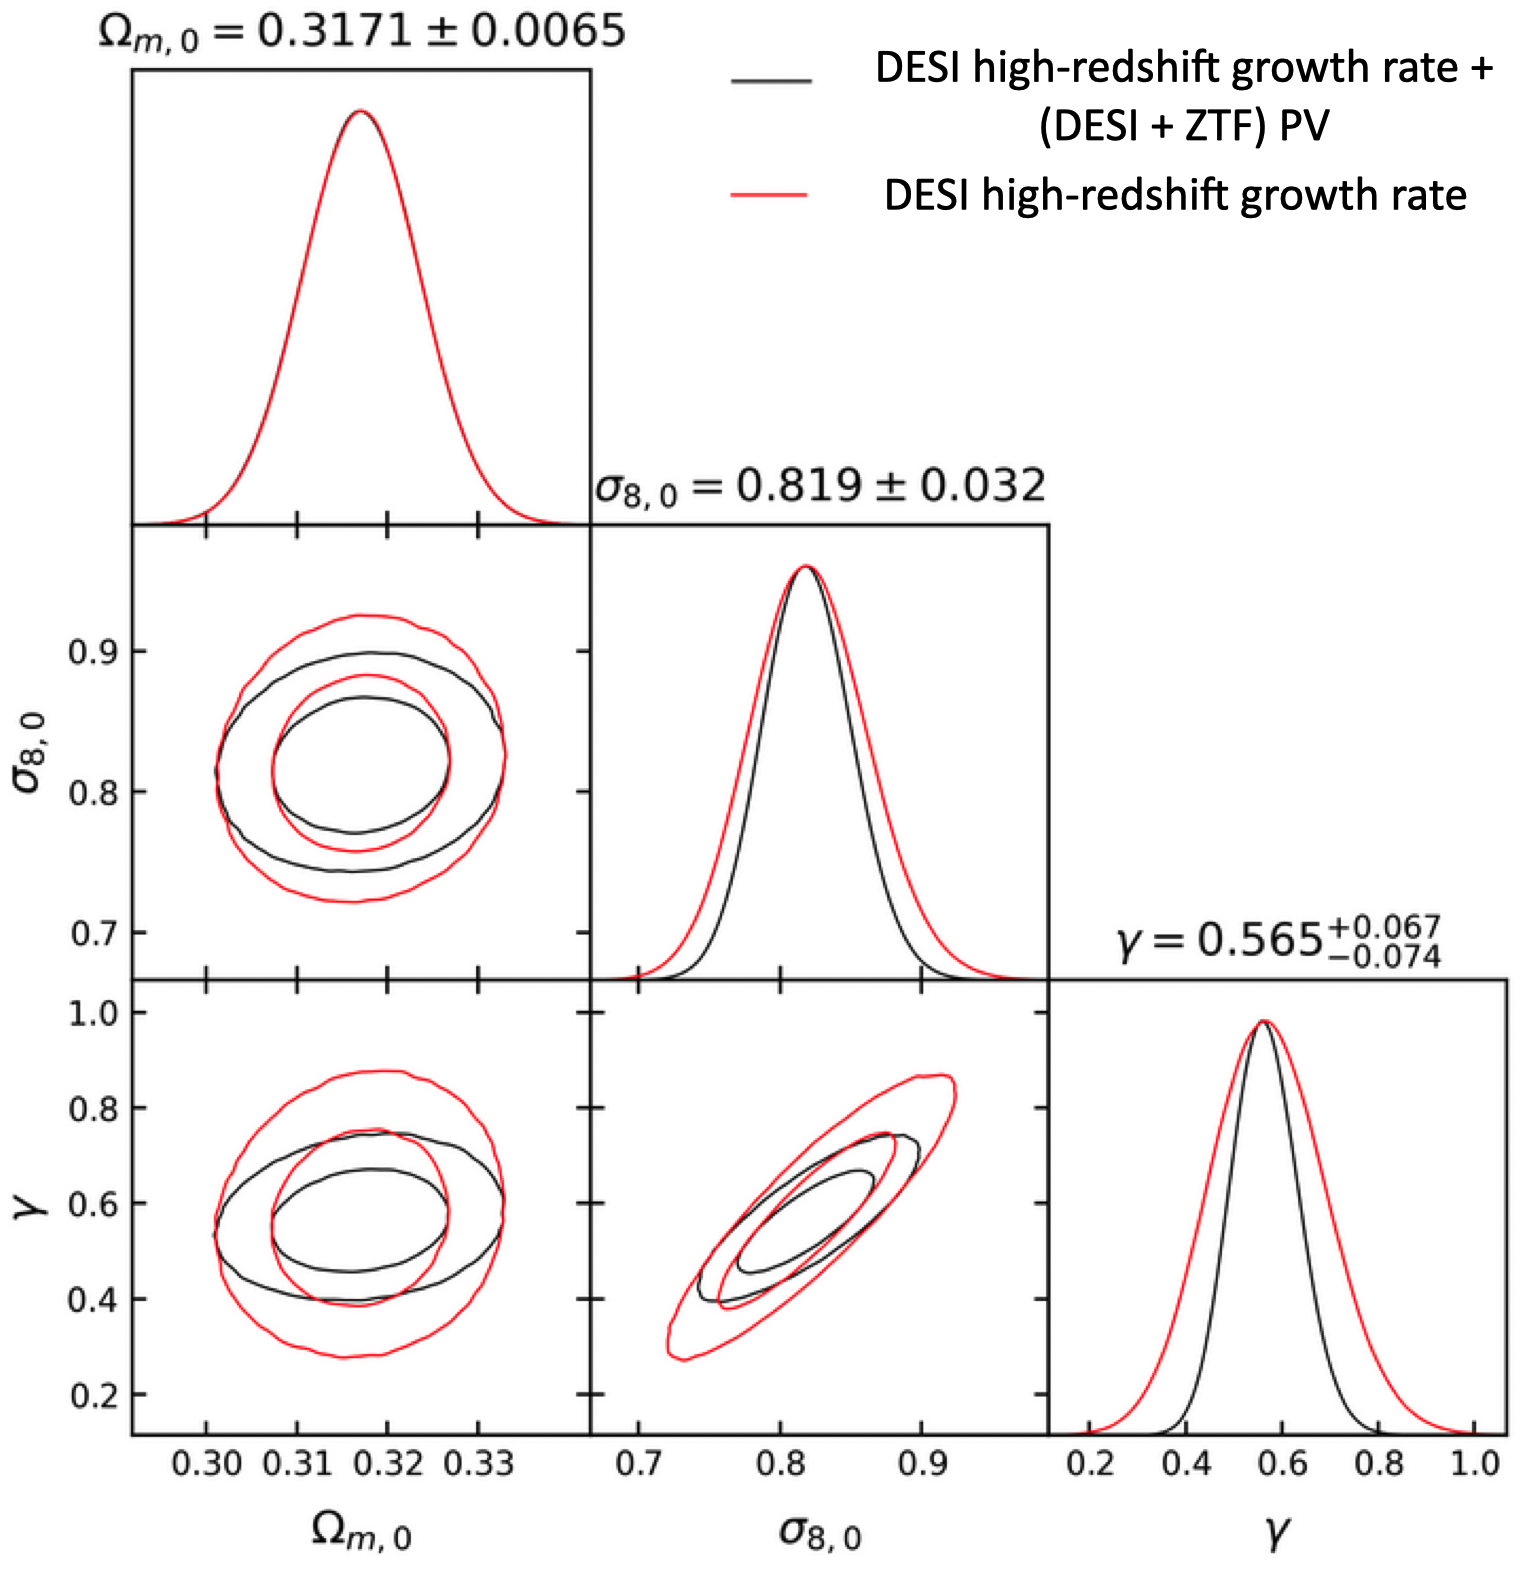
\includegraphics[width=0.6\textwidth]{figures/gamma.png}
    \caption{Forecasted constraints on $\gamma$, $\sigma_8$ and $\Omega_m$ 
    from the final DESI growth rate measurements at high-redshift ($z>0.1$, red lines)
    and when adding our low-redshift growth rate measurement from DESI and ZTF peculiar velocities (black lines).}
    \label{fig:gamma}
  \end{figure}
  
  
  We will also explore the $(\mu_0, \Sigma_0)$ model 
  which empirically parametrize deviations from general relativity at the level 
  of Poisson equations. This parametrization is interesting when combining 
  growth rate measurements with weak-lensing ones, which are orthogonal in this 
  parameter space. Results from WP2 will particularly useful, since it will be 
  necessary to account for the correlations between growth rate measurements from 
  peculiar velocities and those from weak lensing. 
  
  Those results will set the tightest constraints from the Northen sky. 
  This work serve as basis for future analyses of datasets in the Southern sky such as 
  Rubin LSST and the 4-meter Multi-Object Spectroscopic Telescope. 

\paragraph{Risk management}

  WP3 requires the completion of WP1 and WP2, therefore there is a \textbf{medium level 
  of risk}, encompassing risks of each work pacakge and potential delays in the 
  execution of \projacro. Given that this project is a collaborative work, 
  there will be a team of people outside \projacro\ that will help pushing 
  those analyses to completion. 